% Provenance (never printed): see sources/outline_sources.md and sources/book1/BRIEFS.md (g5/02).
\chapter{Text, Pictures and Sound as Numbers}\label{ch:g5:text-pictures-sound-as-numbers}

Lina sends a message to her cousin: ``HI''. Her cousin's phone, far away,
shows the two letters a moment later. But no letter travelled along the
cables: what travelled was sixteen \omterm{def:g5:bits-and-bytes:bit}{bits}, sixteen 0s and 1s. A \omterm{def:g1:what-is-a-computer:computer}{computer} keeps
only \omterm{def:g5:bits-and-bytes:bit}{bits}, so a letter, a photo and a song must all become numbers first. This
chapter shows how.

\begin{recall}
A \omterm{def:g5:bits-and-bytes:bit}{bit} is a choice between 0 and 1; a \omterm{def:g4:memory-and-storage:byte}{byte} is eight \omterm{def:g5:bits-and-bytes:bit}{bits} and holds a whole
number from 0 to 255; numbers can be written in \omterm{def:g5:bits-and-bytes:binary}{binary}
(\cref{ch:g5:bits-and-bytes}).
\end{recall}

\section{Every character has a number}

\begin{definition}[Character code]\label{def:g5:text-pictures-sound-as-numbers:code}
A \emph{character code}\index{character code} is the number given to a
character (a letter, a digit, a sign, the space) by a \emph{code
table}\index{code table}, a table agreed by everyone, so that all \omterm{def:g1:what-is-a-computer:computer}{computers}
turn the same character into the same number.
\end{definition}

% ledger: g5:ascii-codes
\begin{center}
\small
\begin{tabular}{*{13}{c}}
\hline
A & B & C & D & E & F & G & H & I & J & K & L & M \\
65 & 66 & 67 & 68 & 69 & 70 & 71 & 72 & 73 & 74 & 75 & 76 & 77 \\
\hline
N & O & P & Q & R & S & T & U & V & W & X & Y & Z \\
78 & 79 & 80 & 81 & 82 & 83 & 84 & 85 & 86 & 87 & 88 & 89 & 90 \\
\hline
\end{tabular}

\smallskip
small letters: a is 97, b is 98, \dots, z is 122 \quad digits: 0 is 48,
1 is 49, \dots, 9 is 57 \quad the space: 32
\end{center}

A word becomes a list of numbers, one for each character, and each number fits
in one \omterm{def:g4:memory-and-storage:byte}{byte}. ``HI'' is 72 and 73; in \omterm{def:g5:bits-and-bytes:binary}{binary}, on one \omterm{def:g4:memory-and-storage:byte}{byte} each, it is 01001000
01001001: sixteen \omterm{def:g5:bits-and-bytes:bit}{bits}.

\begin{omfigure}
\begin{tikzpicture}[x=1cm, y=1cm, font=\small,
    ch/.style={draw=black!60, fill=ocYellow!35, rounded corners=2pt, minimum width=1.2cm, minimum height=0.8cm, font=\Large\bfseries},
    num/.style={draw=black!60, fill=ocBlue!15, rounded corners=2pt, minimum width=1.2cm, minimum height=0.7cm},
    bits/.style={draw=black!60, fill=ocMint!25, rounded corners=2pt, minimum width=2.4cm, minimum height=0.7cm, font=\ttfamily}]
  \node[ch] (h) at (0,2.4) {H}; \node[ch] (i) at (3,2.4) {I};
  \node[num] (h2) at (0,1.2) {72}; \node[num] (i2) at (3,1.2) {73};
  \node[bits] (h3) at (0,0) {01001000}; \node[bits] (i3) at (3,0) {01001001};
  \foreach \a/\b in {h/h2, h2/h3, i/i2, i2/i3} \draw[-{Stealth[length=2mm]}, black!60] (\a) -- (\b);
  \node[anchor=west, font=\footnotesize] at (4.6,2.4) {the characters};
  \node[anchor=west, font=\footnotesize] at (4.6,1.2) {their codes, from the table};
  \node[anchor=west, font=\footnotesize] at (4.6,0) {one byte each: $64 + 8 = 72$, $64 + 8 + 1 = 73$};
\end{tikzpicture}

{\small ``HI'' on its way: characters, then numbers, then \omterm{def:g5:bits-and-bytes:bit}{bits}.}
\label{fig:g5:text-pictures-sound-as-numbers:hi}
\end{omfigure}

\begin{history}[A table agreed by everyone]
% ledger: g5:ascii-1968
The table used here comes from the American code for exchanging information,
known as ASCII, in its version of 1968. It gives numbers to the English
letters, the digits, the signs and a few control codes, 128 characters in all.
Later, a much larger table was made, with a number for every character of every
alphabet, Chinese characters and emoji included; it keeps the same numbers for
the characters of this small table.
\end{history}

\section{A picture is a grid of pixels}

Look at a screen through a magnifying glass: the picture is made of tiny
squares, in rows and columns, each of one single colour.

\begin{definition}[Pixel]\label{def:g5:text-pictures-sound-as-numbers:pixel}
A \emph{pixel}\index{pixel} is one of the tiny squares, all of one colour,
that make up a picture on a screen or in a \omterm{def:g3:files-and-folders:file}{file}, arranged in rows and columns.
\end{definition}

The simplest pictures are black and white: each \omterm{def:g5:text-pictures-sound-as-numbers:pixel}{pixel} is black or white, so
one \omterm{def:g5:bits-and-bytes:bit}{bit} is enough for it, 1 for black and 0 for white.

\begin{omfigure}
\begin{tikzpicture}[x=0.42cm, y=0.42cm, font=\footnotesize]
  \foreach \row [count=\r from 0] in {00111100,01000010,10100101,10000001,10100101,10011001,01000010,00111100} {
    \foreach \c in {0,...,7} {
      \StrChar{\row}{\numexpr\c+1\relax}[\bitc]
      \if1\bitc \fill[black] (\c,-\r) rectangle ++(1,1); \fi
      \node[font=\footnotesize\ttfamily] at (12.5+\c*0.9,-\r+0.5) {\bitc};
    }
  }
  \draw[black!40] (0,-7) grid (8,1);
  \node[font=\footnotesize, anchor=west] at (11.9,-8.2) {rows of bits, from the top};
  \node[font=\footnotesize] at (4,-8.2) {the picture};
\end{tikzpicture}

{\small A smiley of 8 by 8 \omterm{def:g5:text-pictures-sound-as-numbers:pixel}{pixels} and its 64 \omterm{def:g5:bits-and-bytes:bit}{bits}: 1 for a black \omterm{def:g5:text-pictures-sound-as-numbers:pixel}{pixel}, 0 for
a white one, one row of \omterm{def:g5:bits-and-bytes:bit}{bits} for each row of \omterm{def:g5:text-pictures-sound-as-numbers:pixel}{pixels}.}
\label{fig:g5:text-pictures-sound-as-numbers:smiley}
\end{omfigure}

\begin{definition}[Grey level]\label{def:g5:text-pictures-sound-as-numbers:grey}
The \emph{grey level}\index{grey level} of a \omterm{def:g5:text-pictures-sound-as-numbers:pixel}{pixel} is a number from 0 to 255
that tells how light it is: 0 is black, 255 is white, and the numbers between
are greys, darker for small numbers and lighter for large ones.
\end{definition}

A \omterm{def:g5:text-pictures-sound-as-numbers:grey}{grey level} fits in one \omterm{def:g4:memory-and-storage:byte}{byte}. For colours, a screen mixes light.

\begin{definition}[RGB colour]\label{def:g5:text-pictures-sound-as-numbers:rgb}
An \emph{RGB colour}\index{RGB colour} is a colour given by three numbers,
each from 0 to 255: how much red, how much green and how much blue light to
mix.
\end{definition}

\begin{omfigure}
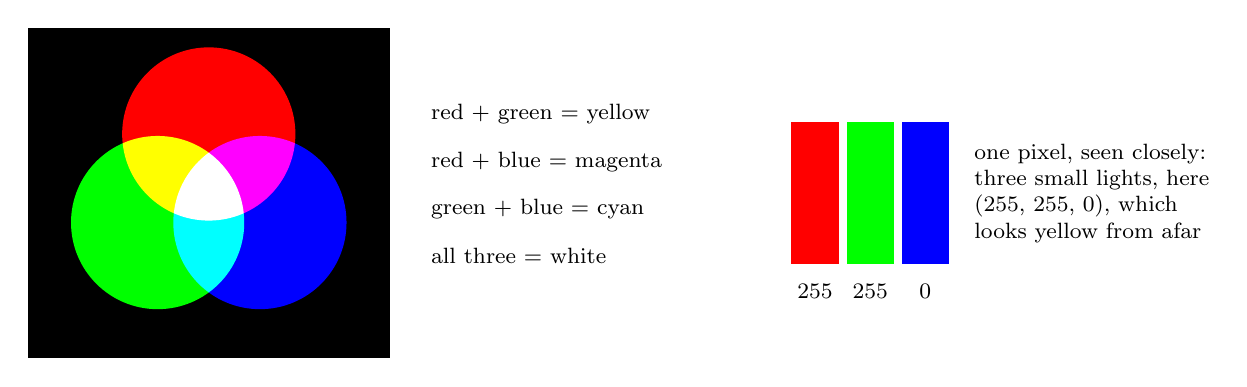
\begin{tikzpicture}[x=1cm, y=1cm, font=\footnotesize]
  \fill[black] (-2.3,-2.1) rectangle (2.3,2.1);
  \begin{scope}[blend group=screen]
    \fill[red] (90:0.75) circle (1.1);
    \fill[green] (210:0.75) circle (1.1);
    \fill[blue] (330:0.75) circle (1.1);
  \end{scope}
  \node[anchor=west, align=left] at (2.7,1.0) {red + green = yellow};
  \node[anchor=west, align=left] at (2.7,0.4) {red + blue = magenta};
  \node[anchor=west, align=left] at (2.7,-0.2) {green + blue = cyan};
  \node[anchor=west, align=left] at (2.7,-0.8) {all three = white};
  \begin{scope}[shift={(7.4,0)}]
    \foreach \c/\n [count=\i] in {red/255, green/255, blue/0} {
      \fill[\c] (0.7*\i-0.7,-0.9) rectangle ++(0.6,1.8);
      \node at (0.7*\i-0.4,-1.25) {\n};
    }
    \node[anchor=west, align=left] at (2.2,0) {one pixel, seen closely:\\three small lights, here\\(255, 255, 0), which\\looks yellow from afar};
  \end{scope}
\end{tikzpicture}

{\small Mixing light. Each \omterm{def:g5:text-pictures-sound-as-numbers:pixel}{pixel} of a screen is three tiny lights, red, green
and blue; the three numbers of the \omterm{def:g5:text-pictures-sound-as-numbers:pixel}{pixel} set how bright each one is.}
\label{fig:g5:text-pictures-sound-as-numbers:rgb}
\end{omfigure}

Mixing light is not like mixing paint: red and green light together look
yellow, and all three at full strength look white. (255, 0, 0) is pure red,
(0, 0, 0) is black, and (255, 255, 255) is white.

\begin{omfigure}
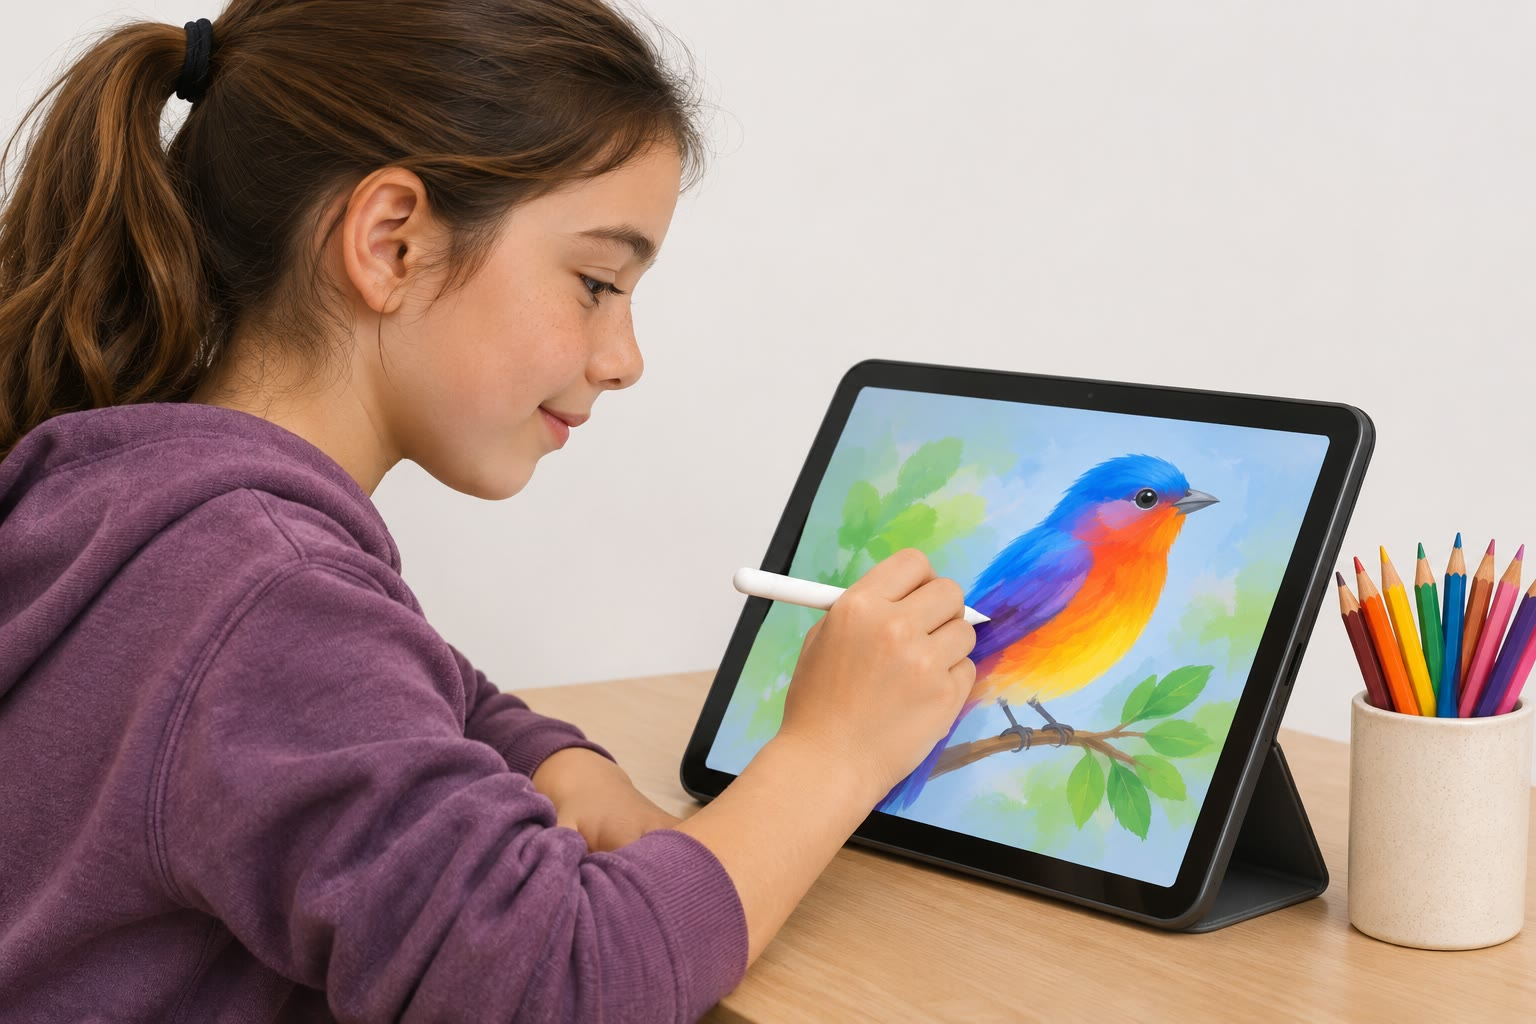
\includegraphics[width=0.48\linewidth]{images/book1/ai/g5-text-pictures-sound-as-numbers-drawing.jpg}

{\small A drawing on a tablet: every stroke changes the three numbers of many
\omterm{def:g5:text-pictures-sound-as-numbers:pixel}{pixels}.}
\end{omfigure}

\section{More pixels, more detail, a bigger file}

\begin{definition}[Resolution]\label{def:g5:text-pictures-sound-as-numbers:resolution}
The \emph{resolution}\index{resolution (of a picture)} of a picture is its
number of \omterm{def:g5:text-pictures-sound-as-numbers:pixel}{pixels}, given as columns by rows: 8 by 8, or \num{1920} by
\num{1080}.
\end{definition}

\begin{omfigure}
\begin{tikzpicture}[x=1cm, y=1cm]
  \begin{scope}
    \foreach \i in {0,...,7} \foreach \j in {0,...,7} {
      \pgfmathtruncatemacro{\in}{((\i+0.5-4)^2+(\j+0.5-4)^2 <= 3.7^2) ? 1 : 0}
      \ifnum\in=1 \fill[ocBlue!80!black] (0.4*\i,0.4*\j) rectangle ++(0.4,0.4); \fi
    }
    \draw[black!30, step=0.4] (0,0) grid (3.2,3.2);
    \node[font=\footnotesize] at (1.6,-0.4) {8 by 8: 64 pixels};
  \end{scope}
  \begin{scope}[shift={(5,0)}]
    \foreach \i in {0,...,31} \foreach \j in {0,...,31} {
      \pgfmathtruncatemacro{\in}{((\i+0.5-16)^2+(\j+0.5-16)^2 <= 15.4^2) ? 1 : 0}
      \ifnum\in=1 \fill[ocBlue!80!black] (0.1*\i,0.1*\j) rectangle ++(0.1,0.1); \fi
    }
    \draw[black!30] (0,0) rectangle (3.2,3.2);
    \node[font=\footnotesize] at (1.6,-0.4) {32 by 32: \num{1024} pixels};
  \end{scope}
\end{tikzpicture}

{\small The same round shape at two \omterm{def:g5:text-pictures-sound-as-numbers:resolution}{resolutions}. With more \omterm{def:g5:text-pictures-sound-as-numbers:pixel}{pixels}, the edge is
smoother; the picture also needs more numbers.}
\label{fig:g5:text-pictures-sound-as-numbers:resolution}
\end{omfigure}

\begin{example}[The size of a picture]\label{ex:g5:text-pictures-sound-as-numbers:size}
A small picture of 400 by 300 \omterm{def:g5:text-pictures-sound-as-numbers:pixel}{pixels} has $400 \times 300 = \num{120000}$
\omterm{def:g5:text-pictures-sound-as-numbers:pixel}{pixels}. Kept as three \omterm{def:g4:memory-and-storage:byte}{bytes} per \omterm{def:g5:text-pictures-sound-as-numbers:pixel}{pixel}, one for each colour, it takes
$\num{120000} \times 3 = \num{360000}$ \omterm{def:g4:memory-and-storage:byte}{bytes}: 360 \omterm{def:g4:memory-and-storage:units}{kilobytes}. Twice as many
columns and twice as many rows make four times as many \omterm{def:g5:text-pictures-sound-as-numbers:pixel}{pixels}, and a \omterm{def:g3:files-and-folders:file}{file} four
times as big.
\end{example}

\section{Sound as a long list of numbers}

Sound is air that shakes back and forth very fast. A microphone turns the
shaking into an electric signal, and the \omterm{def:g1:what-is-a-computer:computer}{computer} measures that signal many
thousands of times every second: each measurement is a number. A song is a very
long list of such numbers. To play it back, the \omterm{def:g1:what-is-a-computer:computer}{computer} sends the numbers to a
speaker, in the same order and at the same speed, and the speaker shakes the
air in the same way: we hear the sound again.

\begin{omfigure}
\begin{tikzpicture}[x=1cm, y=1cm, font=\footnotesize]
  \draw[black!40, -{Stealth[length=2mm]}] (0,0) -- (10.4,0) node[right] {time};
  \draw[ocBlue!80!black, thick, domain=0:10, samples=200] plot (\x, {1.1*sin(\x*72) + 0.35*sin(\x*205)});
  \foreach \k in {0,...,20} {
    \pgfmathsetmacro{\x}{0.5*\k}
    \pgfmathsetmacro{\y}{1.1*sin(\x*72) + 0.35*sin(\x*205)}
    \draw[black!35] (\x,0) -- (\x,\y);
    \fill[ocRed!80!black] (\x,\y) circle (0.06);
  }
\end{tikzpicture}

{\small A sound as a wave (blue) and the measurements a \omterm{def:g1:what-is-a-computer:computer}{computer} keeps (red
dots): one number at each tick of a clock.}
\label{fig:g5:text-pictures-sound-as-numbers:sound}
\end{omfigure}

\section{Everything in a file is bits}

Text, pictures, sounds, films and \omterm{def:g4:programs-and-operating-system:program}{programs} are all kept in the same way: as
numbers, and so as \omterm{def:g5:bits-and-bytes:bit}{bits}. Nothing in a \omterm{def:g3:files-and-folders:file}{file} says ``I am a picture'', apart from
the agreement between the \omterm{def:g4:programs-and-operating-system:program}{program} that wrote it and the \omterm{def:g4:programs-and-operating-system:program}{program} that reads it.
That is why the \omterm{def:g3:files-and-folders:extension}{extension} of a \omterm{def:g3:files-and-folders:file}{file name} matters
(\cref{ch:g3:files-and-folders}): it tells the \omterm{def:g1:what-is-a-computer:computer}{computer} which \omterm{def:g4:programs-and-operating-system:program}{program} knows how
to turn these \omterm{def:g5:bits-and-bytes:bit}{bits} back into letters, colours or sounds.

\section{Exercises}

\begin{exercise}[$\star$]\label{exo:g5:text-pictures-sound-as-numbers:1}
Write the word ``CAT'' as a list of \omterm{def:g5:text-pictures-sound-as-numbers:code}{character codes}.
\end{exercise}

\begin{exercise}[$\star$]\label{exo:g5:text-pictures-sound-as-numbers:2}
Which word do the codes 79 and 75 make?
\end{exercise}

\begin{exercise}[$\star$]\label{exo:g5:text-pictures-sound-as-numbers:3}
Why do ``A'' and ``a'' have different codes?
\end{exercise}

\begin{exercise}[$\star$]\label{exo:g5:text-pictures-sound-as-numbers:4}
Draw the picture of 5 by 5 \omterm{def:g5:text-pictures-sound-as-numbers:pixel}{pixels} given by these rows of \omterm{def:g5:bits-and-bytes:bit}{bits} (1 for black):
00100, 01110, 11111, 01110, 00100.
\end{exercise}

\begin{exercise}[$\star$]\label{exo:g5:text-pictures-sound-as-numbers:5}
What is the \omterm{def:g5:text-pictures-sound-as-numbers:grey}{grey level} of a white \omterm{def:g5:text-pictures-sound-as-numbers:pixel}{pixel}? Of a black one?
\end{exercise}

\begin{exercise}[$\star$]\label{exo:g5:text-pictures-sound-as-numbers:6}
Give the three numbers of a \omterm{def:g5:text-pictures-sound-as-numbers:pixel}{pixel} of pure red, then of pure blue.
\end{exercise}

\begin{exercise}[$\star$]\label{exo:g5:text-pictures-sound-as-numbers:7}
A colour picture of 10 by 10 \omterm{def:g5:text-pictures-sound-as-numbers:pixel}{pixels} is kept with three \omterm{def:g4:memory-and-storage:byte}{bytes} per \omterm{def:g5:text-pictures-sound-as-numbers:pixel}{pixel}. How
many \omterm{def:g4:memory-and-storage:byte}{bytes} does it take?
\end{exercise}

\begin{exercise}[$\star$]\label{exo:g5:text-pictures-sound-as-numbers:8}
Read the third row of \omterm{def:g5:bits-and-bytes:bit}{bits} of the smiley. What part of the face does it draw?
\end{exercise}

\begin{exercise}[$\star\star$]\label{exo:g5:text-pictures-sound-as-numbers:9}
Which colour does the \omterm{def:g5:text-pictures-sound-as-numbers:pixel}{pixel} (255, 255, 0) show? And (0, 255, 255)?
\end{exercise}

\begin{exercise}[$\star\star$]\label{exo:g5:text-pictures-sound-as-numbers:10}
A picture of 100 by 100 \omterm{def:g5:text-pictures-sound-as-numbers:pixel}{pixels} and a picture of 200 by 200 \omterm{def:g5:text-pictures-sound-as-numbers:pixel}{pixels} are kept the
same way. How many times bigger is the second \omterm{def:g3:files-and-folders:file}{file}?
\end{exercise}

\begin{exercise}[$\star\star$]\label{exo:g5:text-pictures-sound-as-numbers:11}
The digit 7 is a character too. Its code is not 7: what is it? Why can the code
of a digit not simply be the digit itself?
\end{exercise}
